\section{Discussion: Rearrangements of Infinite Series}
    Consider the infinite series
    \begin{equation*}
        \sum_{n=1}^\infty\frac{(-1)^{n+1}}{n} = 1 - \frac{1}{2} + \frac{1}{3} - \frac{1}{4} + \frac{1}{5} - \frac{1}{6} + \dots 
    \end{equation*}
    If we just add from left to right, we get a series of \textit{partial sums}: $s_1 = 1,\; s_2 = 1/2,\; s_3 = 5/6$, and so on. We also see that the sums oscillate such that $s_1 > s_3 > s_5 > \dots$ and $s_2 < s_4 < s_6 < \dots$.
    \begin{center}
        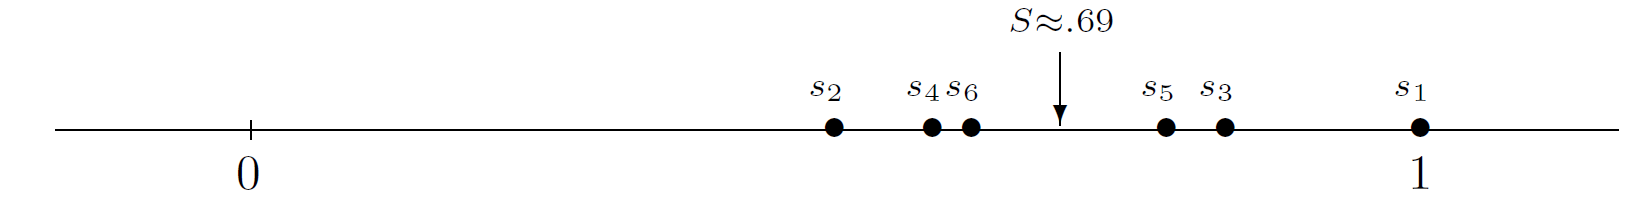
\includegraphics[width=200pt]{oscillating_converging.png}
    \end{center}
    \begin{equation*}
        s_2 < s_4 < s_6 < \dots < S < \dots < s_5 < s_3 < s_1
    \end{equation*}
    It is reasonable to say that this series converges to a number $S = 0.69$ (by experimentation with $s_N$ where $N$ is a large number). It is tempting to think that the sum of all those numbers "add" up to $S$, but for that we must redefine addition for infinite sums. Treating this series algebraically, lets multiply through by $1/2$ and add it back.
    \begin{center}
        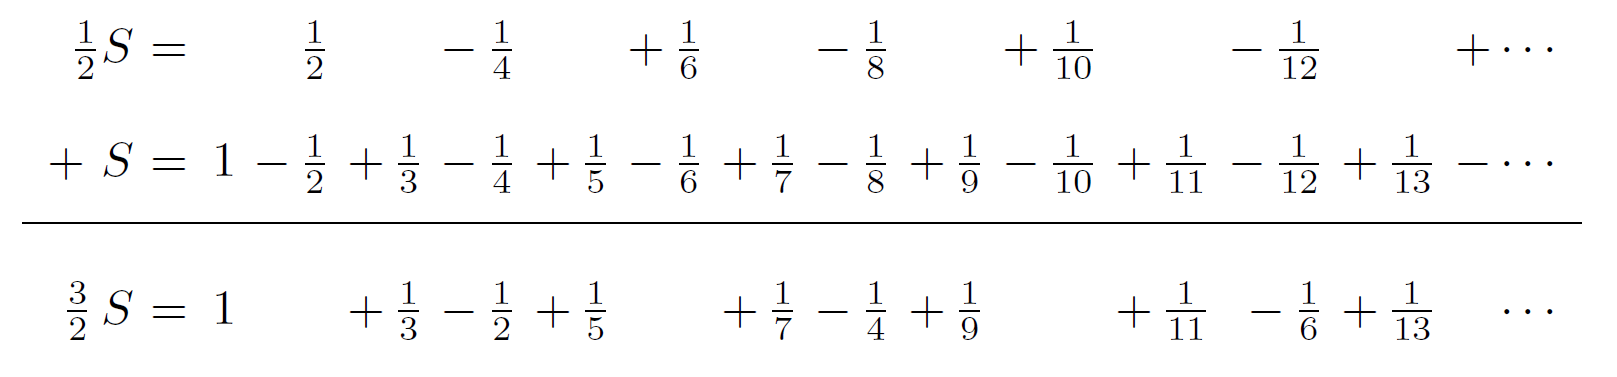
\includegraphics[width=300pt]{communitive.png}
    \end{center}
    The resulting series has the same terms as the original series except in a different order. It has two positive terms and then the negative term instead of switching each time. But $\frac{3}{2}S \neq S$. This is also seen by experimentation with large $N$s. Addition, in this infinite setting, is not commutative.
    \newline \indent
    Let us look at another series
    \begin{equation*}
        \sum_{n=0}^\infty (-1/2)^n
    \end{equation*}
    Using $\sum_{n=0}^\infty r^n = \frac{1}{1 - r}$ for geometric series, we get
    \begin{equation*}
        1 - \frac{1}{2} + \frac{1}{4} - \frac{1}{8} + \frac{1}{16} - \frac{1}{32} + \dots = \frac{1}{1 - 1/2} = \frac{2}{3}
    \end{equation*}
    If we rearrange this into two positive and then a negative, you get the same result. Hence addition in an infinite setting is sometimes commutative.
    \newline \indent
    This is applied to the double summation of numbers in a \textit{grid}. For example, ${a_{ij}: i, j \in \textbf{N}}$, where $a_{ij} 1/2^{j - i}$ if $j > i$, $a_{ij} = -1$ if $j = i$, and $a_{ij} = 0$ if $j < i$.
    $$
        \mqty[
            -1 & \frac{1}{2} & \frac{1}{4} & \frac{1}{8} & \frac{1}{16} & \dots \\[10pt]
            0 & -1 & \frac{1}{2} & \frac{1}{4} & \frac{1}{8} & \dots \\[10pt]
            0 & 0 & -1 & \frac{1}{2} & \frac{1}{4} & \dots
        ]
    $$
    We are trying to give
    \begin{equation*}
        \sum_{i,j=1}^\infty a_{ij}
    \end{equation*}
    mathematical meaning. If we sum over all of the $j$ while holding $i$ for each row we get
    \begin{equation*}
        \sum_{i,j=1}^\infty a_{ij} = \sum_{i=1}^\infty(\sum_{j=1}^\infty a_{ij}) = \sum_{i=1}^\infty 0 = 0
    \end{equation*}
    since the sum of each row is zero. If we hold $j$ constant and iterate over $i$ first we get
    \begin{equation*}
        \sum_{i,j=1}^\infty a_{ij} = \sum_{j=1}^\infty(\sum_{i=1}^\infty a_{ij}) = \sum_{j=1}^\infty (\frac{-1}{2^{j-1}}) = -2
    \end{equation*}
    The order in which we add causes us to get different results. This double summation occurs when we are multiplying two series:
    \begin{equation*}
        \sum a_i \sum b_j = \sum_{i,j} a_ib_j
    \end{equation*}
    Now consider the associative property of addition. Consider $\sum_{n=1}^\infty (-1)^n$.
    \begin{equation*}
        \sum_{n=1}^\infty (-1)^n = (-1 + 1) + (-1 + 1) + (-1 + 1) + (-1 + 1) + (-1 + 1) + \dots = 0
    \end{equation*}
    \begin{equation*}
        \sum_{n=1}^\infty (-1)^n = -1 +(1 - 1) + (1 - 1) + (1 - 1) + (1 - 1) + (1 - 1) + \dots = -1
    \end{equation*}
    Different associations cause use to get different results. Manipulations that are legitimate in finite settings do not always extend to infinite settings.